\paragraph{GET /:lang}
\begin{itemize}
\item \textbf{Successo}:\\
Questo scenario rappresenta il successo di una richiesta di keywords inerenti alla lingua impostata che impone, come vincolo per poter essere effettuata, che l'utente non sia autenticato e non possieda già un account nel sistema.  
\label{Procedura di traduzione}
\begin{figure}[ht]
	\centering
	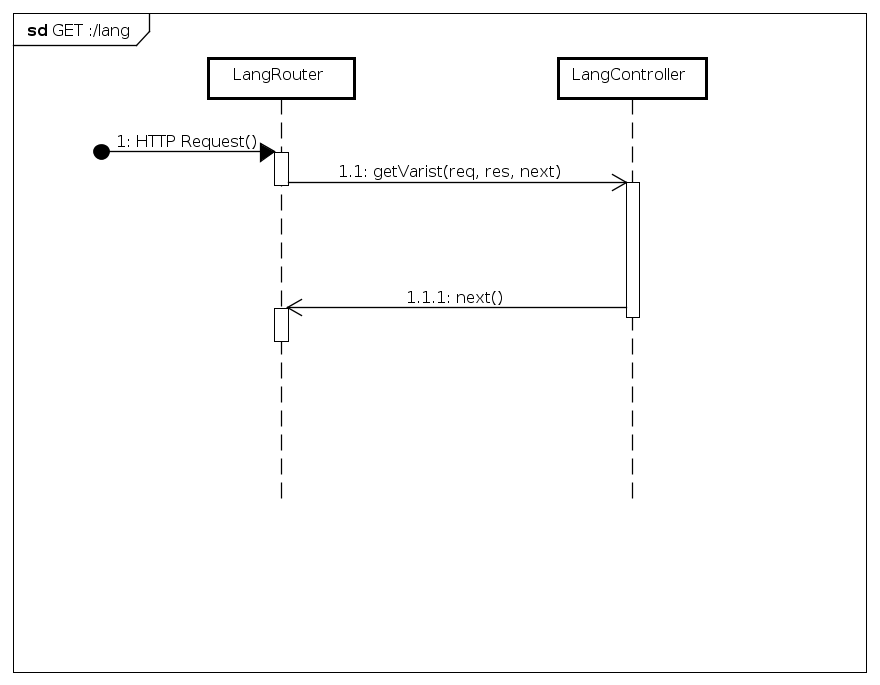
\includegraphics[scale=0.40]{UML/DiagrammiDiSequenza/Back-end/GET_lang_success.png}
	\caption{GET /:lang}
\end{figure}
\FloatBarrier

\item \textbf{Fallimento}:\\
Quando viene effettuata una richiesta di traduzione in una lingua non riconosciuta dal sistema viene sollevato un errore. Tale scenario rappresenta il fallimento di una richiesta di traduzione che impone, come vincolo per poter essere effettuata, che l'utente non sia autenticato e non possieda già un account nel sistema. In questo caso il modulo \texttt{LangController} invia \texttt{next(error)} per il fallimento di tale vincolo al router il quale avrà compito di reinstradarlo (indirizzandolo verso \texttt{ErrorHandler}).
 
\label{Fallimento della procedura di traduzione}
\begin{figure}[ht]
	\centering
	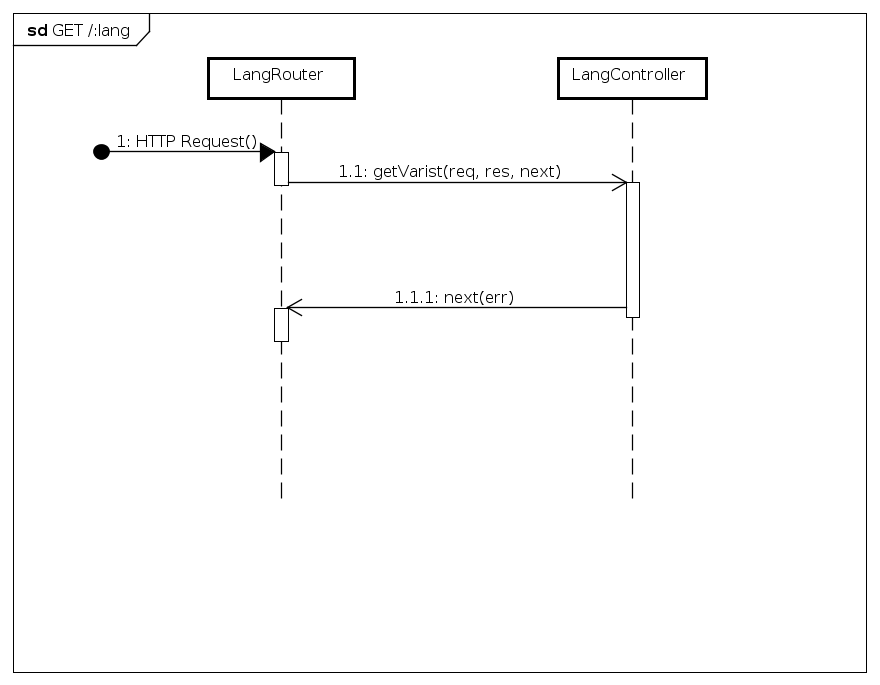
\includegraphics[scale=0.40]{UML/DiagrammiDiSequenza/Back-end/GET_lang_failure.png}
	\caption{GET /:lang}
\end{figure}
\FloatBarrier
\end{itemize}


\paragraph{POST /:lang/signup}
\begin{itemize}
\item \textbf{Successo}:\\
Questo scenario rappresenta il successo di una richiesta di registrazione che impone, come vincolo per poter essere effettuata, che l'utente non sia autenticato e non possieda già un account nel sistema. La registrazione dell'utente nel sistema viene effettuata tramite \textit{Passport\ped{G}} creando ed inserendo un nuovo \textit{document} all'interno della collection User.

\label{Procedura di registrazione}
\begin{figure}[ht]
	\centering
	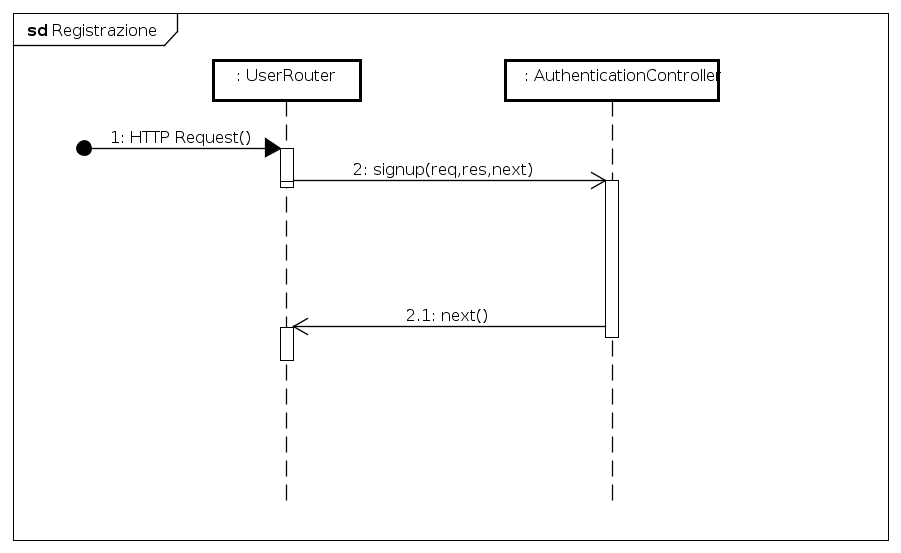
\includegraphics[scale=0.40]{UML/DiagrammiDiSequenza/Back-end/POST__lang_signup_success.png}
	\caption{POST /:lang/signup}
\end{figure}
\FloatBarrier

\item \textbf{Fallimento}:\\
Quando un utente effettua una richiesta di registrazione e cerca di inserire dei dati già presenti del \textit{database\ped{G}} viene sollevato un errore. Tale scenario rappresenta il fallimento di una richiesta di registrazione che impone, come vincolo per poter essere effettuata, che l'utente non sia autenticato e non possieda già un account nel sistema. In questo caso il modulo \texttt{AuthenticationController} invia \texttt{next(error)} per il fallimento di tale vincolo al router il quale avrà compito di reinstradarlo (indirizzandolo verso \texttt{ErrorHandler}).

\label{Fallimento della procedura di registrazione}
\begin{figure}[ht]
	\centering
	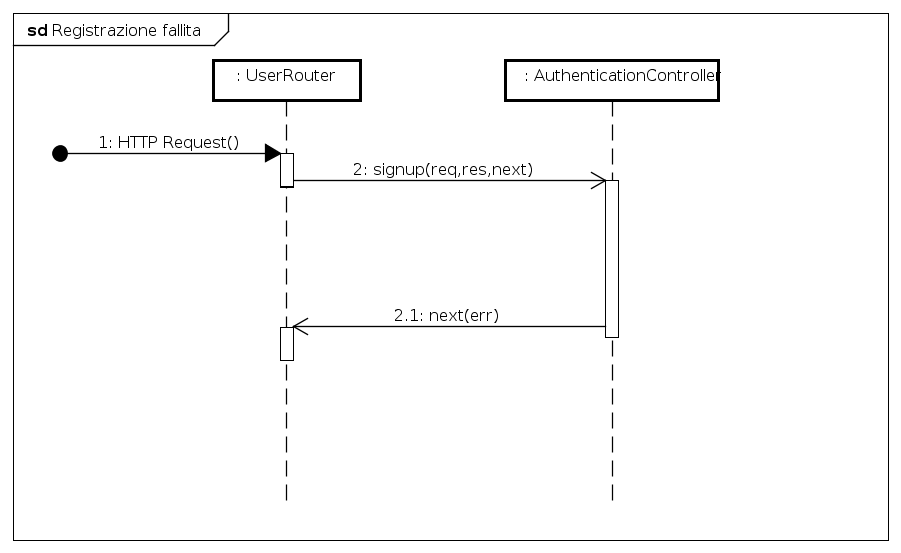
\includegraphics[scale=0.40]{UML/DiagrammiDiSequenza/Back-end/POST__lang_signup_failure.png}
	\caption{Fallimento della procedura di registrazione}
\end{figure}
\FloatBarrier

\end{itemize}

\paragraph{POST /:lang/signin}
\begin{itemize}
\item \textbf{Successo}:\\
La maggior parte delle richieste alle risorse rese disponibili dalle \textit{API\ped{G}} del \textit{server\ped{G}} possono essere effettuate solamente da un \textit{utente autenticato}. Tale scenario rappresenta il successo di una richiesta di \textit{login}, che impone come vincolo per poter essere effettuata, che l'utente abbia un account nel sistema, ma che non sia già autenticato. La \textit{login} dell'utente viene effettuata tramite \textit{Passport\ped{G}}.

\label{Procedura di autenticazione}
\begin{figure}[ht]
	\centering
	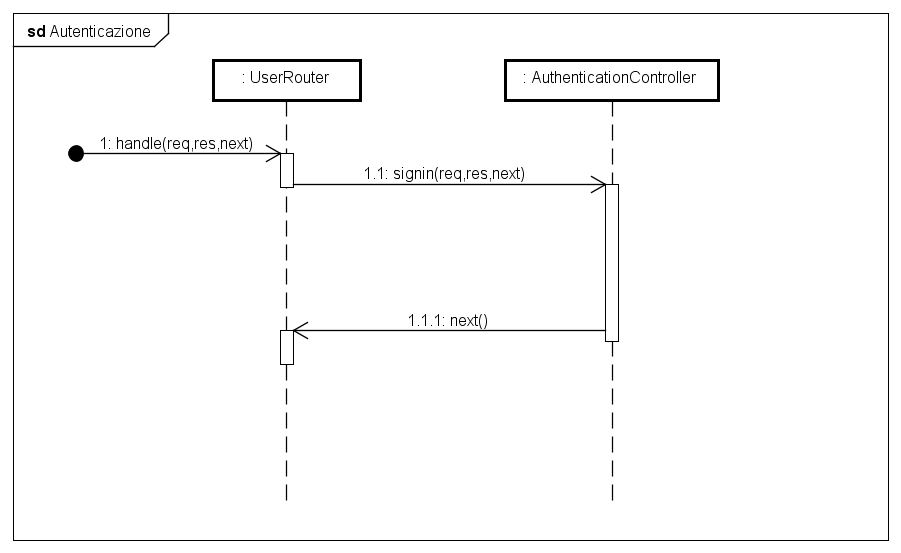
\includegraphics[scale=0.40]{UML/DiagrammiDiSequenza/Back-end/POST__lang_signin_success.png}
	\caption{POST /:lang/signin}
\end{figure}
\FloatBarrier
 
\item \textbf{Fallimento}:\\
La maggior parte delle richieste alle risorse rese disponibili dalle \textit{API\ped{G}} del \textit{server\ped{G}} possono essere effettuate solamente da un \textit{utente autenticato}. Tale scenario rappresenta il fallimento della richiesta di \textit{login}, che può avvenire nel caso sia stia cercando di autenticare un utente non registrato. In questo caso il modulo \texttt{AuthenticationController} invia \texttt{next(error)} al router, il quale avrà compito di reinstradarlo (indirizzandolo verso \texttt{ErrorHandler}).

\label{Fallimento della procedura di autenticazione}
\begin{figure}[ht]
	\centering
	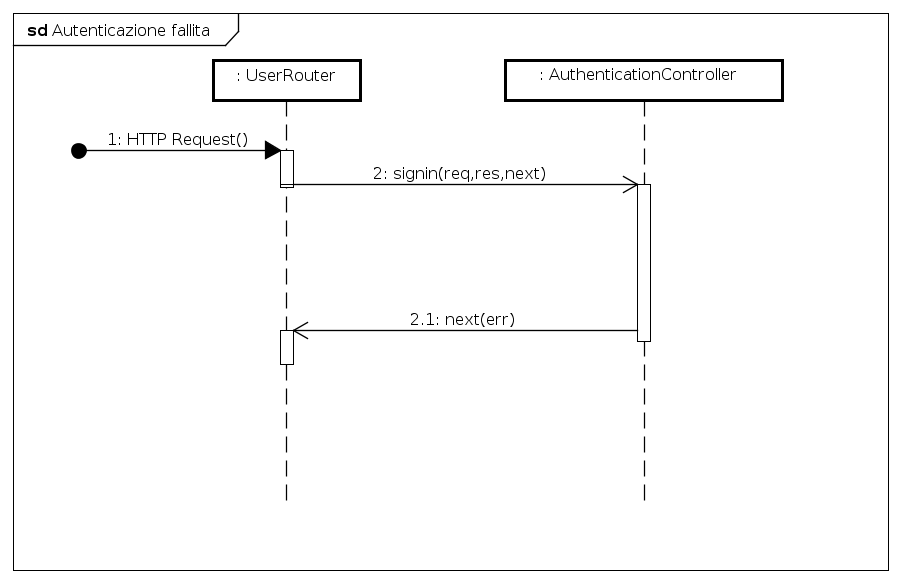
\includegraphics[scale=0.40]{UML/DiagrammiDiSequenza/Back-end/POST__lang_signin_failure.png}
	\caption{Fallimento della procedura di autenticazione}
\end{figure}
\FloatBarrier

\end{itemize}

\paragraph{POST /:lang/signout}
\begin{itemize}
\item \textbf{Successo}
% descrizione diagramma e UML
\item \textbf{Fallimento}
% descrizione diagramma e UML
\end{itemize}

\paragraph{GET /:lang/loggedin}
\begin{itemize}
\item \textbf{Successo}:\\
Questo scenario rappresenta il successo di una richiesta di controllo di sessione che non impone alcun vincolo per poter essere effettuata. Il controllo di sessione dell'utente nel sistema viene effettuata tramite il modulo \texttt{SessionController} che invia \texttt{next()} al router, per indicare il successo dell'operazione .

\label{Procedura di controllo di sessione}
\begin{figure}[ht]
	\centering
	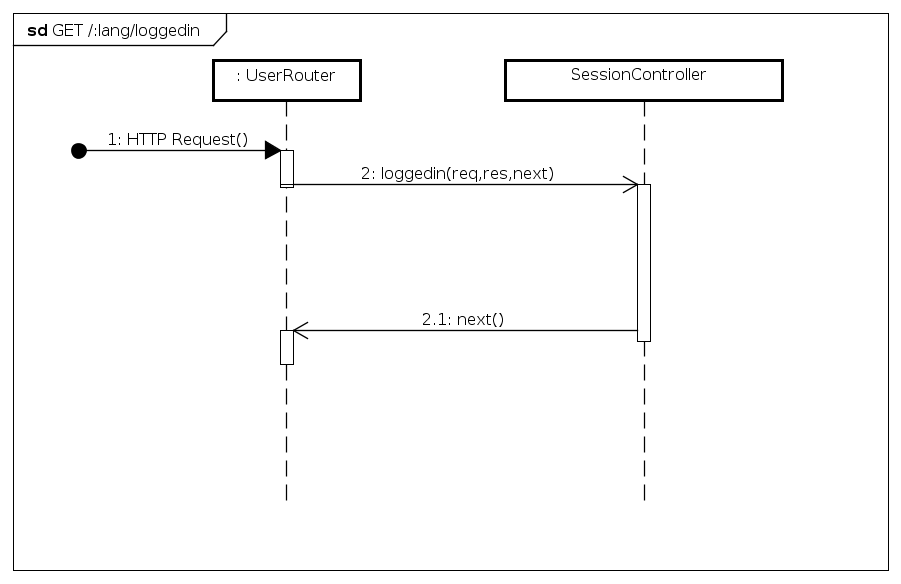
\includegraphics[scale=0.40]{UML/DiagrammiDiSequenza/Back-end/GET__lang_loggedin_success.png}
	\caption{Procedura di controllo di sessione}
\end{figure}
\FloatBarrier
 
\item \textbf{Fallimento}:\\
Questo scenario rappresenta il fallimento di una richiesta di controllo di sessione che non impone alcun vincolo per poter essere effettuata. Il controllo di sessione dell'utente nel sistema viene effettuata tramite il modulo \texttt{SessionController}, che in caso di fallimento, invia \texttt{next(err)} al router,  il quale avrà compito di reinstradarlo (indirizzandolo verso \texttt{ErrorHandler}).

\label{Fallimento della procedura di controllo di sessione}
\begin{figure}[ht]
	\centering
	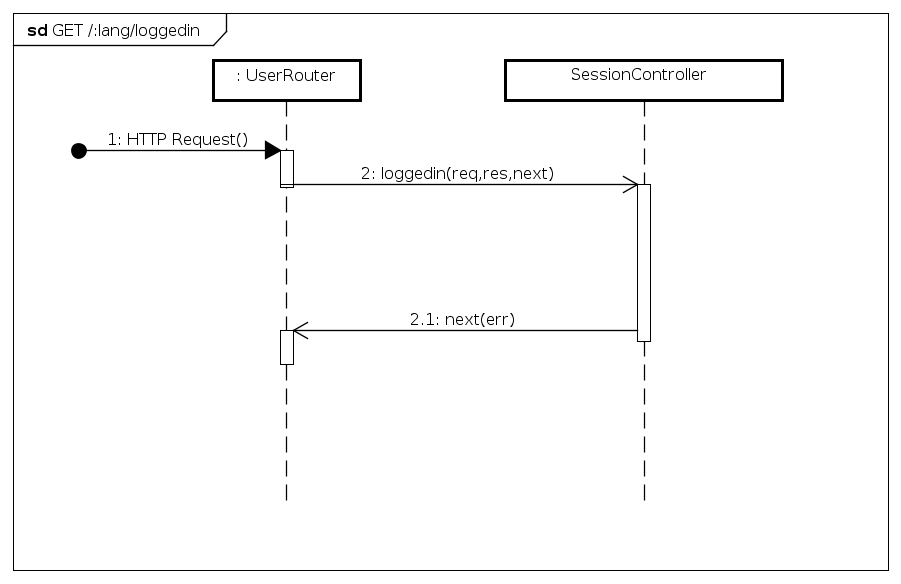
\includegraphics[scale=0.40]{UML/DiagrammiDiSequenza/Back-end/GET__lang_loggedin_failure.png}
	\caption{Fallimento della procedura di controllo di sessione}
\end{figure}
\FloatBarrier

\end{itemize}

